\chapter{Meta Feature Extraction}
\label{chap:class}

The first addition to SNOOKER: A DataSet GeNeratOr fOr HelpdesK SERvices was the inclusion of a meta feature extraction model. The objective was to allow users to extract meta features from the generated datasets, making it possible to extrapolate the quality of the synthetic data. It was also essential to enable meta-extraction of other datasets, making the product usable for meta-extraction tasks for datasets external to the generation.

Past development of the generator was made using Python. As the meta-extraction feature was idealized as an increment to the current product, it used the same language and foundation.

The evolution of this advancement proved quite troublesome; the development steps and the results are described in this chapter.

\section{Meta feature extraction}
Development started with manually coding the extraction of meta features from small (about 100 rows) synthetic datasets. A list of meta features to be included in the analysis was made, considering the information acquired in Chapter \ref{chap:mf}.

Testing started with the simple meta feature analysis of a dataset. As the generator creates synthetic datasets in a .csv (Comma-separated values) format, a way to analyse such data was necessary. One major issue for would-be statistical Python programmers in the past has been the lack of libraries implementing standard models and a cohesive framework for specifying models. Pandas\footnote{\href{https://pandas.pydata.org/}{pandas.pydata.org}} is a Python library of rich data structures and tools for working with structured data sets. It is commonly used in statistics, finance, social sciences, and many other fields \citep{mckinney2011pandas}. It intends to close the gap in the richness of available data analysis tools between Python, general-purpose systems and scientific computing language, and the numerous domain-specific statistical computing platforms and database languages. Pandas was therefore used.

General meta feature analysis was relatively simple to implement due to being directly observable from the dataset, representing basic information and being the most explicit set in terms of computation cost. Problems arrived when looking at the analysis of statistical meta features. 

The development of models to analyse every statistical meta feature was slow. Continuing down that path would limit the scope of the work given the existing time frame and delivery dates. The solutions available were to limit the number of analysed meta features (extracting only a hand full per family) or to rely on external tools to perform that same task. The latter option was chosen. After consideration, the Python library Python Meta Feature Extractor (pyfme\footnote{\href{https://pymfe.readthedocs.io/en/latest/index.html}{pymfe.readthedocs.io}}) was selected and used to perform meta feature extraction tasks.

The pymfe library provides a comprehensive set of meta features implemented in python. According to the library developers, the package brings cutting-edge meta features, following recent literature proposals. The pymfe architecture was idealised to systematically make the extraction, which can produce a robust set of meta features. The review performed by \cite{alcobacca2020mfe} agreed with our decision and proved a suitable validator. As such, development moved forth using this library.

Pymfe can extract several families of meta features from a dataset. Those families are depicted in the following list, with tables describing every family's meta feature presented in Appendix \ref{ap1:pymfe_mf}.
\begin{itemize}
  \item \textbf{General}: General information related to the dataset, also known as simple measures, such as the number of instances, attributes and classes (Table \ref{tab:pymfe-general-mf}).
  \item \textbf{Statistical}: Standard statistical measures to describe the numerical properties of data distribution (Table \ref{tab:pymfe-statistical-mf}).
  \item \textbf{Information-theoretic}: Particularly appropriate to describe discrete (categorical) attributes and their relationship with the classes (Table \ref{tab:pymfe-it-mf}).
  \item \textbf{Model-based}: Measures designed to extract characteristics from simple machine learning models (Teable \ref{tab:pymfe-mb-mf}).
  \item \textbf{Landmarking}: Performance of simple and efficient learning algorithms (Table \ref{tab:pymfe-landmarking-mf}).
  \item \textbf{Relative Landmarking}: Relative performance of simple and efficient learning algorithms.
  \item \textbf{Subsampling Landmarking}: Performance of simple and efficient learning algorithms from a subsample of the dataset.
  \item \textbf{Clustering}: Clustering measures extract information about dataset based on external validation indexes (Table \ref{tab:pymfe-clustering-mf}).
  \item \textbf{Concept}: Estimate the variability of class labels among examples and the examples density (Table \ref{tab:pymfe-concept-mf}).
  \item \textbf{Itemset}: Compute the correlation between binary attributes (Table \ref{tab:pymfe-itemset-mf}).
  \item \textbf{Complexity}: Estimate the difficulty in separating the data points into their expected classes (Table \ref{tab:pymfe-complexity-mf}).
\end{itemize}

The vast amount of families and collections of meta features inside those families proved more than enough to use in our meta-extraction model. Some limitations were, however, applied. Pandas is unable to analyse datasets with missing data. Meta features that use missing data as a parameter had to be left out.

Right in the start, the library requires the definition and extraction of the first column from the dataset to analyse CSV data. The definition of the column name can be surpassed using pandas' ability to read information from CSV data. The program can automatically grab the first column from a dataset. The generator already creates an expendable 'ID' column in its first position, which can be consumed without affecting the meta feature analysis result. However, this does not apply to other possible datasets, forcing users to edit datasets not generated by SNOOKER to get valid results. The snippet \ref{lst:pandas} shows an example of code used to read the CSV file while consuming the first column.

\par\noindent\rule{\textwidth}{0.4pt}
\begin{lstlisting}[language=Python, caption=Importing the csv dataset with ID column, label={lst:pandas}]
  df = pd.read_csv(path, sep=";", index_col=False)
  X, y = df.drop(df.columns[0], axis=1), df[df.columns[0]]
\end{lstlisting}
\par\noindent\rule{\textwidth}{0.4pt}

Another simple limitation was defining a sep for the CSV data. In the case of SNOOKER, CSV is generated using semi-colons, which was the used value for steps.

The meta-extraction feature was intended as the main addition to SNOOKER. It needed to be integrated into the generator's interface, making it possible to be accessible to users in a simple way. The development of the interface will be tackled in the next section.

Each meta feature family selected outputs a file at the end of the analysis. This file contains the path to the analysed dataset, the results of each meta feature inside that family and the time it took to perform that meta feature extraction. A transcription of an actual output file from a meta feature extraction analysis can be found in Appendix \ref{ap2:meta_files}.

\section{Interface}
The Meta Feature Extraction Module was always idealized as an increment made to SNOOKER during this study. As such, it needed a user interface to allow user-module interaction. An interface was created and appended to the generator's frontend. As seen in Chapter \ref{chap:Problem}, SNOOKER's interface was developed using PyQt, which meant that this interface had to be developed using the same technology.

"Python is probably the easiest to learn and nicest scripting language in widespread use, and Qt is probably the best library for developing GUI applications. The combination of Python and Qt, "PyQt", makes it possible to develop applications on any supported platform and run them unchanged on all supported platforms" (quoted from \cite{summerfield2007rapid}).

%PyQt5 is the latest version of a GUI widgets toolkit developed by Riverbank Computing. It is a Python interface for Qt, one of the most powerful, and popular cross-platform GUI library. PyQt5 is a blend of Python programming language and the Qt library.

The interface went through an idealization period, and the concept and objectives changed. Originally the interface was supposed to have a button that would trigger a file selection. This selection would generate a series of rows containing that file's column names. Next to each column name, we would have a toggle feature to select columns to use in the calculations. It would also be accompanied by a dropdown containing options to select the data type in that column (Numeral, Text, Date, etc.). The concept for the original interface can be found in Figure \ref{fig:class_original_interface}. 

\begin{figure}[t]
  \begin{center}
    \leavevmode
    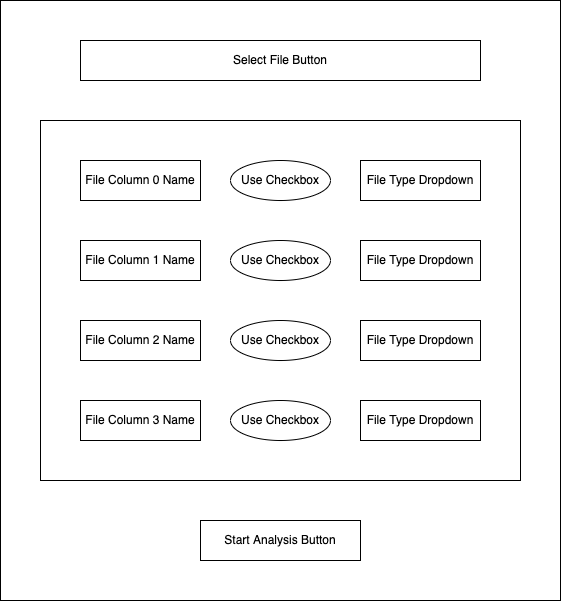
\includegraphics[width=0.5\textwidth]{original_idea.png}
    \caption{Original idealization of meta-extraction feature interface}
    \label{fig:class_original_interface}
  \end{center}
\end{figure}

The meta feature calculations were coded by hand, using a series of measures requiring user input on each column's data type. The system could not distinguish between categorical and numeric features, creating error breaks in the analysis. Although implementation started, it was quickly dropped, and no visual record was kept of its development.

When moving to the pymfe library, the interface changed to focus on more relevant features, the selection of meta features. The current implementation keeps the file selection button. Still, it forgoes the column toggle and data type selection, using a simple toggle of meta feature families. Figure \ref{fig:class_interface_2} depicts the final interface. 



\begin{figure}[!h]
  \begin{center}
    \leavevmode
    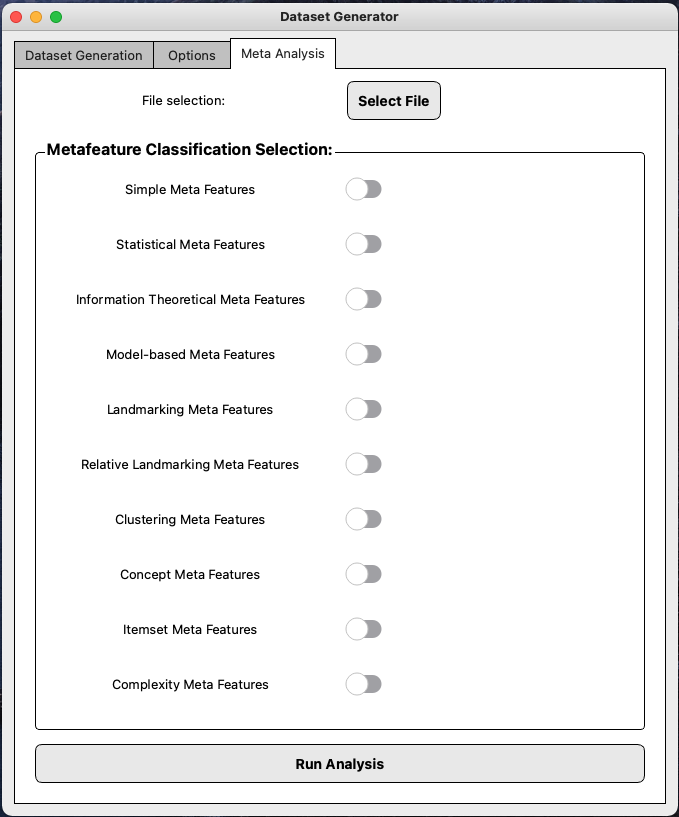
\includegraphics[width=0.6\textwidth]{interface_class_2.png}
    \caption{Meta Feature Extraction feature interface }
    \label{fig:class_interface_2}
  \end{center}
\end{figure}

\section{Library Limitations}
Opting to use the pymfe library proved to be the right choice, as it propelled the development of a large number of steps. It was possible to classify datasets with a giant gallery of meta features. However, some limitations were accompanied by the library. 

One such limitation was quickly found: the time needed to perform meta feature extraction analysis. While small datasets took only a few minutes to analyse, as the size of the dataset increased, so did the time the analysis took to finish. Several tests were made and data extracted to see what families of meta features were causing the output delay. That data can be found in Table \ref{tab:analysis_time}. It should be noted that way more tests were made during the development of this study. Nonetheless, results were sometimes incomplete and/or used datasets with different amounts of columns. The datasets chosen to perform this first analysis were all generated by SNOOKER.

\begin{table}[h!]
  \centering
  \caption{Testing made on the meta-extraction feature, using several datasets. }
  \setlength{\tabcolsep}{8pt}
    \renewcommand{\arraystretch}{1.2}
      \begin{tabular}{llllll}
        \hline
        Meta Feature family     & DS1       & DS2       & DS3       & DS4       & DS5 \\ \hline
        Simple                  & 2.21s     & 3.25s     & 6.27s     & 11.90s    & 32.70s\\
        Statistical             & 28:16 min & 17:06 min & 12.22 min & >2h       & 51:31 min\\
        Information Theoretical & 24.82s    & 21.9s     & 45.72s    & 43.55s    & 1:26 min\\
        Model-based             & 4.47s     & 1:15 min  & 25:42 min & >2h       & >2h \\
        Landmarking             & <1s       & 2.69s     & 5.34s     & 23.07 s   & 38.73s \\
        Relative Landmarking    & 6.25s     & 2.19s     & 5.23s     & 17:06 min & >2h \\
        Clustering              & 3:13 min  & 4:29 min  & 13:19 min & 45:23min  & >2h \\
        Concept                 & 8.52s     & 29.02s    & 58.32s    & 52.15s    & 57.46s\\
        Itemset                 & 5.14 min  & 10:38 min & 23:57 min & >2h       & >2h\\
        Complexity              & >4h       & >4h       & >4h       & >4h       & >4h \\\hline
  \end{tabular}
  \label{tab:analysis_time}
\end{table}

DS1, DS2, DS3 and DS4 were SNOOKER-generated datasets with 1000, 2000, 3000, 4000 and 5000 entries, respectively. Some outliers can be found on datasets with more entries where certain calculations took way more time than the rest. Many outliers can be attributed to hardware limitations. Overheating and memory problems were faced when leaving the meta-extractor module running for hours. However, we can see that statistical analysis took more time than any other analysis. Complexity analysis was also incapable of reaching any result, even having double the available time limit to perform said analysis. Initially, the sentiment was that hardware limitations were accountable for these analysis times. Yet, when testing the meta-extraction feature on a much more powerful machine, the end result times were similar to those achieved locally. It could then be concluded that the statistical and complexity times problem was not the computational power. 

Regular analysis was kept running for a maximum amount of 2 hours per meta family. However, complexity analysis took way more time from the beginning. We tried to see how far we could go on their research, making 2 tests with 2 different datasets with a time limit of 12 hours. Both these tests were unable to lead to results. We then tried using datasets with a low number of entries. This analysis's result is displayed in Table \ref{tab:small_analysis_time}. We used 5 SNOOKER-generated datasets with 100, 200, 300, 400 and 500 entries. We compared the time it took to perform a statistical analysis (the second most time-consuming analysis) to the time taken by complexity calculations. On that same table, we also have a Ratio row. This ratio indicates the $ComplexityTime/StatisticalTime$ relation.
\begin{table}[b]
  \centering
  \caption{Complexity and Statistical runtimes on small datasets}
  \setlength{\tabcolsep}{8pt}
    \renewcommand{\arraystretch}{1.2}
      \begin{tabular}{llllll}
        \hline
        Entries     & 100       & 200       & 300       & 400       & 500 \\ \hline
        Statistical & 1.5s      & 10.60s    & 38.52s    & 1:25 min  & 2:55 min \\
        Complexity  & 53.62s    & 5:53 min  & 17:46 min & 40:17 min  & 1:24:53 h \\\hline\hline
        Ratio       & 35.75     & 33.30     & 27.67     & 28.44     & 29.01\\\hline
  \end{tabular}
  \label{tab:small_analysis_time}
\end{table}

From the analysis, we could conclude that Complexity analysis took way too much time to complete compared to other meta-calculations. Further investigation of these meta features was dropped as time constraints made their study impossible to pursue. The option to analyse them is still present in the current product. However, due to the limitations mentioned earlier, its use is not recommended on local machines.

While Complexity Meta-Analysis was dropped from further development. The same could not apply to Statistical Meta Features as their values are some of the most important we could extract from a dataset. So what if we could remove some meta features from the module? The idea was to test each statistical meta feature extraction. We would save each analysis's time and remove more time-consuming meta features, making the calculation faster. 

We used the previously used SNOOKER-generated datasets to get the statistical analysis times. However, it soon became obvious that it would take too much time. Complete statistical analysis of SD1 took more than 15 hours to complete (the output of this analysis can be seen in Appendix \ref{appendix:statistical}). We decided to use a series of smaller, publicly available datasets\footnote{\href{https://perso.telecom-paristech.fr/eagan/class/igr204/datasets}{perso.telecom-paristech.fr}}. Several other datasets were also used in the analysis, but as dataset dimensionality grew, so did time required to analyse all 19 meta features plus the full analysis. Runtime of each analysis is presented in Table \ref{tab:stat_analysis_time}.

\begin{table}[t!]
  \centering
  \caption{Statistical meta analysis duration}
  \setlength{\tabcolsep}{8pt}
    \renewcommand{\arraystretch}{1.2}
      \begin{tabular}{llllll}
        \hline
        Meta Feature  & SD1   & cars & cereal & CausesOfDeath\_France\_2001-2008 \\ \hline
        can\_cor      & 26:32 min &50.97s & 0.48s & 13:07 min \\
        cor & 27:16 min & 52.99s & 0.46s & 12:31 min\\
        cov & 25:29 min & 52.40s & 0.46s & 12:25 min \\
        eigenvalues & 31:03 min & 52.54s & 0.47s & 11:25 min \\
        g\_mean & 25:42 min & 52.55s & 0.46s & 11:37 min \\
        gravity & 26:54 min & 52.16s & 0.45s & 11:38 min \\
        h\_mean & 25:32 min & 52.11s & 0.45s & 11:38 min \\
        iq\_range & 27:45 min & 1:44 min & 0.46s & 11:31 min\\
        kurtosis & 26:54 min & 1:07 min & 0.51s & 11:36 min\\
        lh\_trace & 26:04 min & 54.09s & 0.45s & 11:34 min\\
        mad & 28:52 min & 52.51s & 0.45s& 11:34 min\\
        max & 26:29 min & 52.51s & 0.44s & 11:34 min\\
        mean & 26:56 min & 51.85s & 0.44s & 11:36 min\\
        median & 27:36 min & 51.88s & 0.44s & 11:33 min\\
        min & 26:31 min & 51.57s & 0.45s & 11:31 min\\
        nr\_cor\_attr & 47:58 min & 51.03s & 0.44s & 11:29 min\\
        nr\_disc & 27:54 min & 50.70s & 0.44s & 11:30 min\\
        nr\_norm & 27:40 min & 51.09s & 0.45s & 11:29 min \\
        nr\_outliers & 24:35 min & 50.99s & 0.44s & 11:33 min\\
        p\_trace & 24:35 min& 50.77s & 0.44a& 11:35 min\\
        range & 35:49 min & 51.02s & 0.44s & 11:35 min\\
        roy\_root & 26:51 min& 52.16s & 0.44s & 11:36 min\\
        sd & 26:14 min & 51.04s & 0.45s & 11:40 min\\
        sd\_ratio & 27:26 min & 50.71s & 0.45s & 11:37 min\\
        skewness & 24:42 min & 50.95s & 0.49s & 12:05 min\\
        sparsity & 27:49 min & 50.67s & 0.42s & 11:24 min \\
        t\_mean & 25:17 min & 50.95s & 0.43s & 11:13 min\\
        var & 24:23 min & 51.76s & 0.42s & 11:10 min\\
        w\_lambda & 23:56 min & 50.65s & 0.43s & 11:08 min\\
        FULL ANALYSIS & 28:16 min& 51.44s & 62.65s & 11:25 min\\
        \hline
  \end{tabular}
  \label{tab:stat_analysis_time}
\end{table}

The outcome of this analysis was unexpected. Even with some calculations taking more time, the differences are predominantly negligible. In fact, the last row shows that the library takes roughly the same time to perform a complete analysis as it does on every individual meta-extraction computation. With this result, proceeding with analysing more enormous datasets proved unnecessary.

Further exploration of the pymfe library proved that improving the calculations it made would be a daunting task. Pymfe was developed by \citet*{alcobacca2020mfe} the leading experts in the field regarding meta analysis. A full review of the library found on kandii\footnote{\href{https://kandi.openweaver.com/python/ealcobaca/pymfe}{https://kandi.openweaver.com/} - kandi is a code and library review website} also showed that the library is of the highest quality. Its most significant flaws were its high code complexity (9614 lines of code, 461 functions and 56 files) and lack of current releases (it had no major release in the last 12 months). As code complexity directly impacts the maintainability of the code, trying to influence its results would require more time and resources than what was available. We were left with no choice but to accept the high wait times when researching some meta feature families.

While abandoning problematic families could alleviate the problem, it would not solve it. Even general meta feature extraction could take a long time to complete, given a large enough dataset. In fact, even problematic familes can achieve results in smaller datasets. Ultimately, looking at the tool as a product, we find it more beneficial to leave the choice up to the end user than to remove it outright.

The meta-extraction module was considered finished with the decision that no further improvements could be made.

\section{Conclusion}
In this chapter, we took a look at the development process for the meta feature extraction module, created as an addition to SNOOKER. We started the chapter by displaying our path until we arrived at an agreeable solution for the meta feature extraction problem. After trying to make all the calculations ourselves, we used the pymfe library to accelerate the process, adding an enormous amount of meta features to the analysis pool.

In the second section, we explore the development of the module's interface, developed using PyQt5. The interface went through a series of alterations and experimentations until we arrived at the current presentable stage.

Lastly, we did some experiments on the final product, identifying problems and finding a way to correct them. Unfortunately, no way to solve the detected problems was found.

Ultimately the Meta-extraction feature ended up going further than what was initially planned. The original concept was to develop this meta-analysis from scratch, getting only some examples from each family. Ultimately, pyfme allowed us not to get some meta feature results but tens of results per analysis. On the matter of optimization, the feature does, however, underperform.